\documentclass[12pt]{article}
\usepackage{enumitem}
\usepackage{mathtools}
\usepackage{amsthm}
\usepackage{graphicx}
\graphicspath{ {images/} }
\begin{document}

\title{Assignment 10}
\author{Darwin Ding}
\maketitle

\section*{Exercise 6.1}
\begin{enumerate}[label=(\alph*)]
	\item Consider a circle centered on the origin. Put two points on the circle such that the line segment between them is a diameter of the circle. Each of these points represents a vector. Clearly, by cosine similarity, these points are as far apart as they could be, as the angle between the vectors is a full 180 degrees. However, as you shrink the radius of the circle the Euclidean distance will decrease more and more. After sufficient shrinkage, you'll be left with a situation where the two vectors are completely dissimilar by cosine similarity, but very similar by Euclidean distance.
	\\ \\ Consider two vectors with a single feature that differs by very little. Both cosine similarity and Euclidean distance will say these two vectors are the same. If you were to add additional features to both vectors that are identical to the feature already there, you would find that the cosine similarity would not change but the Euclidean distance would continue to get larger and larger. With sufficient features, Euclidean distance will say these vectors are very dissimilar but cosine similarity will not agree.
	\item Cosine similarity will change with changes in the origin. Euclidean distance is just the raw differences between all of the components of both vectors, so if the origin shifts all of the components will individually shift in the same way. However, cosine similarity is defined as the angular distance between two vectors, and if you change where the origin is, the vectors' angles from the origin will change.
	\\ \\ In general, cosine similarity would be the best metric to pick for the job. Euclidean distance is very fickle and implementation heavy, and naturally decreases with an increasing number of features because it's a simple sum.
\end{enumerate}

\section*{Exercise 6.2}
\begin{enumerate}[label=(\alph*)]
	\item First, the gradient descent function was set to have step size 0.01 and run for 50 iterations starting from $(0.1, 0.1)$. The following plot of iterations vs. $f(x)$ was created:
	\\ 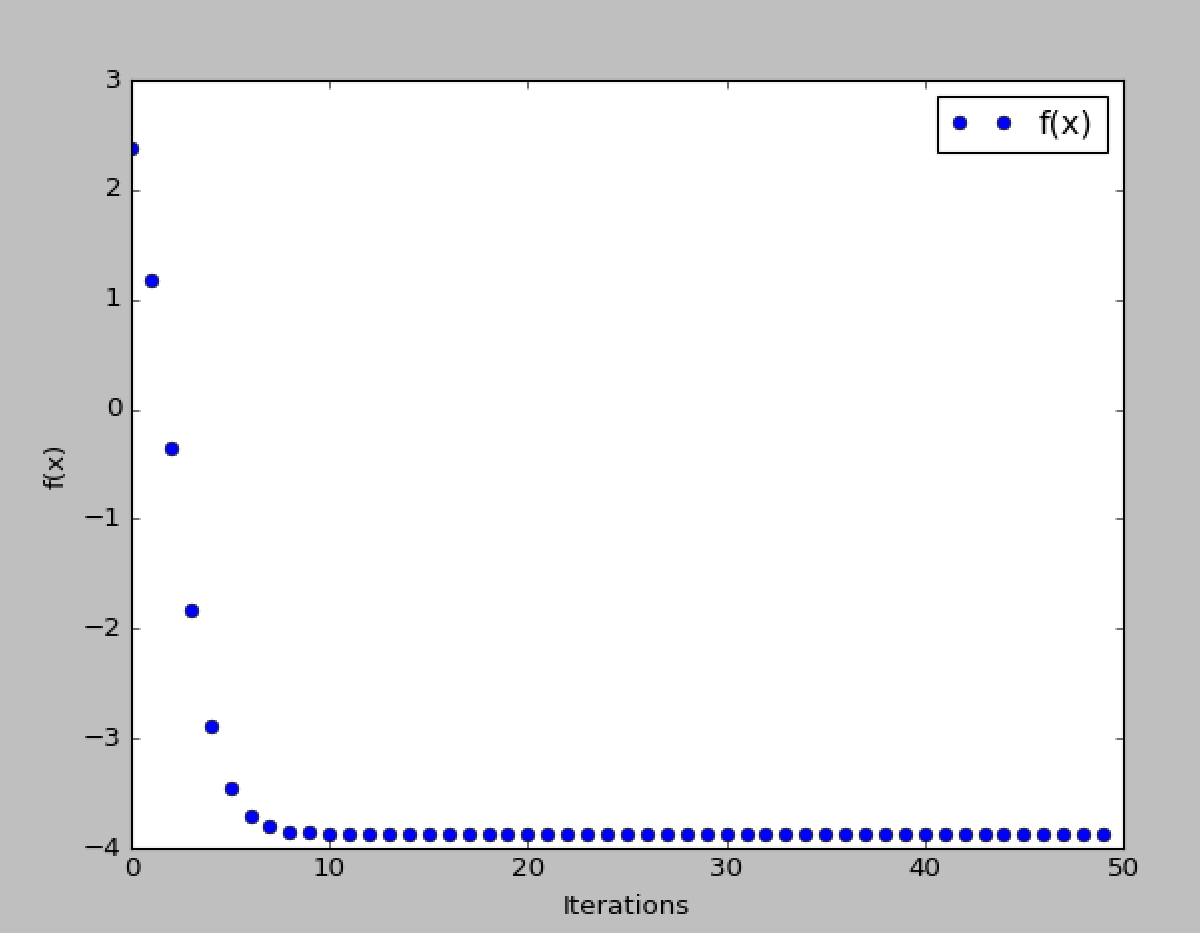
\includegraphics[scale=.5]{2a1.png}
	\\ The final algorithm outputted the point: $\boldsymbol{(-0.238, -0.238)}$ with a final $f(x)$ of $\boldsymbol{-3.88}$
	\\ \\ Then, the step size was changed to 0.1 and rerun with the same number of iterations and starting point, creating the following plot:
	\\ 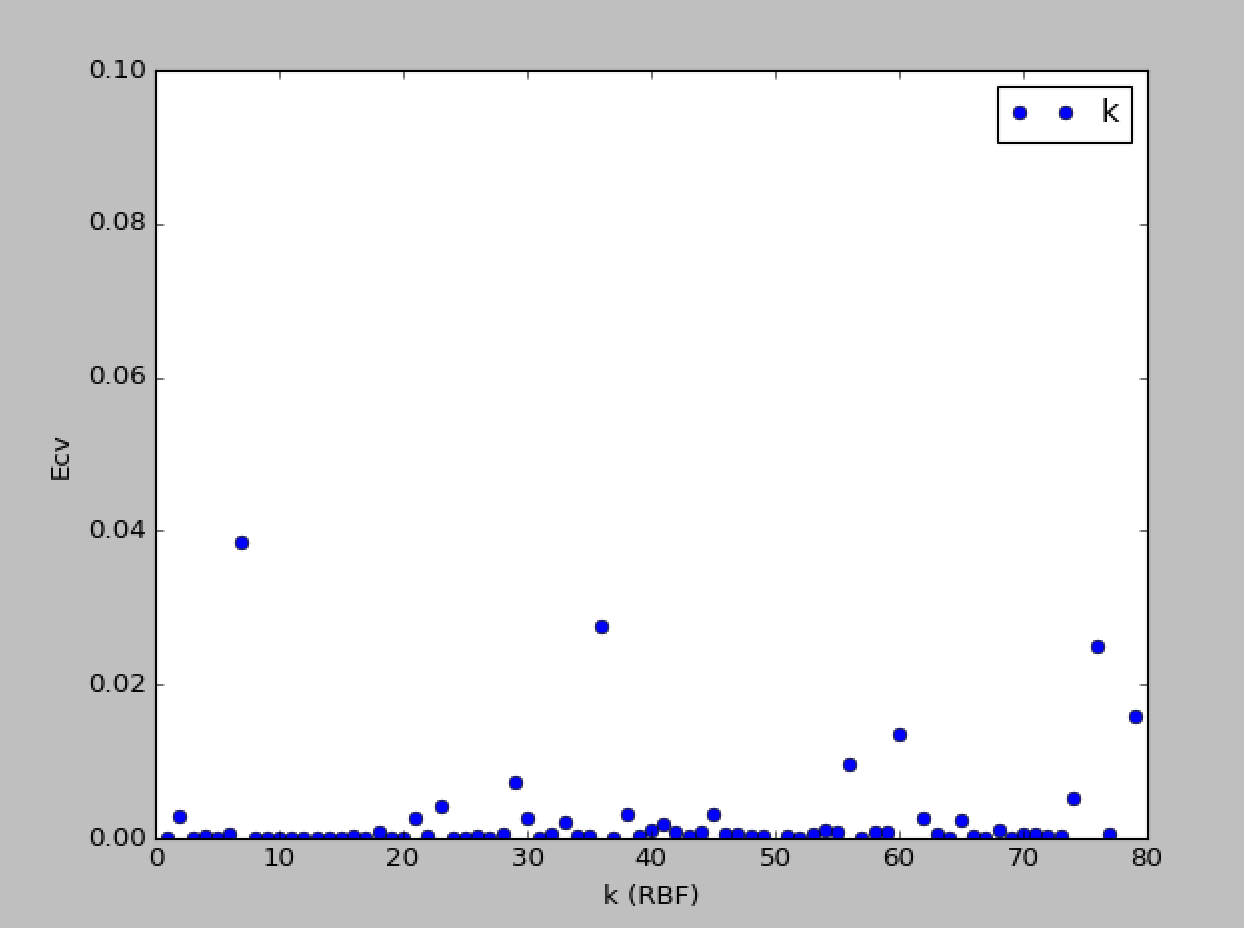
\includegraphics[scale=.5]{2a2.png}
	\\ The final algorithm outputted the point: $\boldsymbol{(-0.0011, -0.0011)}$ with a final $f(x)$ of $\boldsymbol{3.28}$. This is clearly wildly wrong, especially considering it is pretty easy to come up with any number lower ($f(0, 0) = 0^2 + 0^2 + 2 sin(0) + 2 sin(0) = 0$, for instance). This happens because the step size is too large. The gradient descent algorithm sees a local gradient then overreacts by jumping all the way over to another part of the plot.
	\item The gradient descent algorithm was then run on a variety of starting points with both step sizes (0.1, 0.01), and the final f(x)s are listed below in the table. Each time, the algorithm was run for 50 iterations.
	\begin{center}
		\begin{tabular}{| l | l | l |}
			\hline
			\textbf{Starting Pt} & $\eta = \boldsymbol{0.01}$ & $\eta = \boldsymbol{0.1}$ \\ \hline
			$(0.1, 0.1)$ & $-3.88$ & $3.28$ \\ \hline
			$(1, 1)$ & $-2.88$ & $-0.5$ \\ \hline
			$(-0.5, -0.5)$ & $-3.88$ & $-3.43$ \\ \hline
			$(-1, -1)$ & $-0.88$ & $3.88$ \\
			\hline
		\end{tabular}
	\end{center}
	Clearly this is all over the place, and the only reason we know that $-3.88$ is probably the lowest is because we were lucky earlier in choosing starting points.
\end{enumerate}

\section*{Problem 3.16}
\begin{enumerate}[label=(\alph*)]
	\item The expected cost of something happening is equal to its cost multiplied by the probability of it happening. Fortunately, we are given both of those as logistic regression outputs probabilities from 0 to 1.
	\\ \\ We only incur an accept cost if the algorithm was wrong on a specific data point $x$. The probability of this happening is $1 - g(x)$, because we computed $g(x)$ to be the probability of the person being correct. As a result, $cost(accept) = [1 - g(x)]c_a$.
	\\ \\ Similarly, we only incur a reject cost if the algorithm was wrong on a specific data point. The probability of this happening is $g(x)$, because we computed $1 - g(x)$ to be the probability of the person being an intruder. As a result, $cost(reject) = g(x)c_r$.
	\item We should put the threshold at the $g(x)$ value where the costs are equal. This is because if, for any of the data points, either of the costs is larger, we should clearly go with that option.
	\begin{gather*}
		cost(reject) = cost(accept)
		\\ (1 - g(x)) c_a = g(x) c_r
		\\ c_a - g(x) c_a = g(x) c_r
		\\ g(x) (c_r + c_a) = c_a
		\\ g(x) = \frac{c_a}{c_r + c_a}
	\end{gather*}
	\item For the Supermarket, $c_a = 1$ and $c_r = 10 \implies \kappa = \frac{c_a}{c_a + c_r} = \frac{1}{1 + 10} = \boldsymbol{\frac{1}{11}}$
	\\ \\ For the CIA, $c_a = 1000$ and $c_r = 1 \implies \kappa = \frac{c_a}{c_a + c_r} = \frac{1000}{1000 + 1} = \boldsymbol{\frac{1000}{1001}}$
\end{enumerate}
\end{document}